\chapter{Testing e validazione}
\label{cha:test}
La fase di testing consiste nella verifica del codice implementato tramite vari casi di test. In generale sono presenti due metodi di testing: l'analisi statica e l'analisi dinamica. Il primo tipo ricerca eventuali errori o comportamenti inaspettati senza eseguire il software stesso, ma solamente analizzandone il codice; la seconda metodologia consiste nella ricerca di malfunzionamenti del prodotto eseguendo il programma con vari input in ingresso prestabiliti. \\
L'analisi dinamica prevede due sottotipi di fasi di verifica e validazione: l'analisi funzionale, che si basa sulla quantità dei test effettuati, e quella strutturale, che invece considera la copertura del codice da testare.
Se quindi l'analisi funzionale ha lo scopo di sottoporre a una serie di casi di test il programma per verificare i requisiti definiti, l'analisi strutturale esegue una serie di casi di test al fine di verificare la maggior quantità possibile di righe di codice.\\

\begin{figure}[!hbt]
\centering
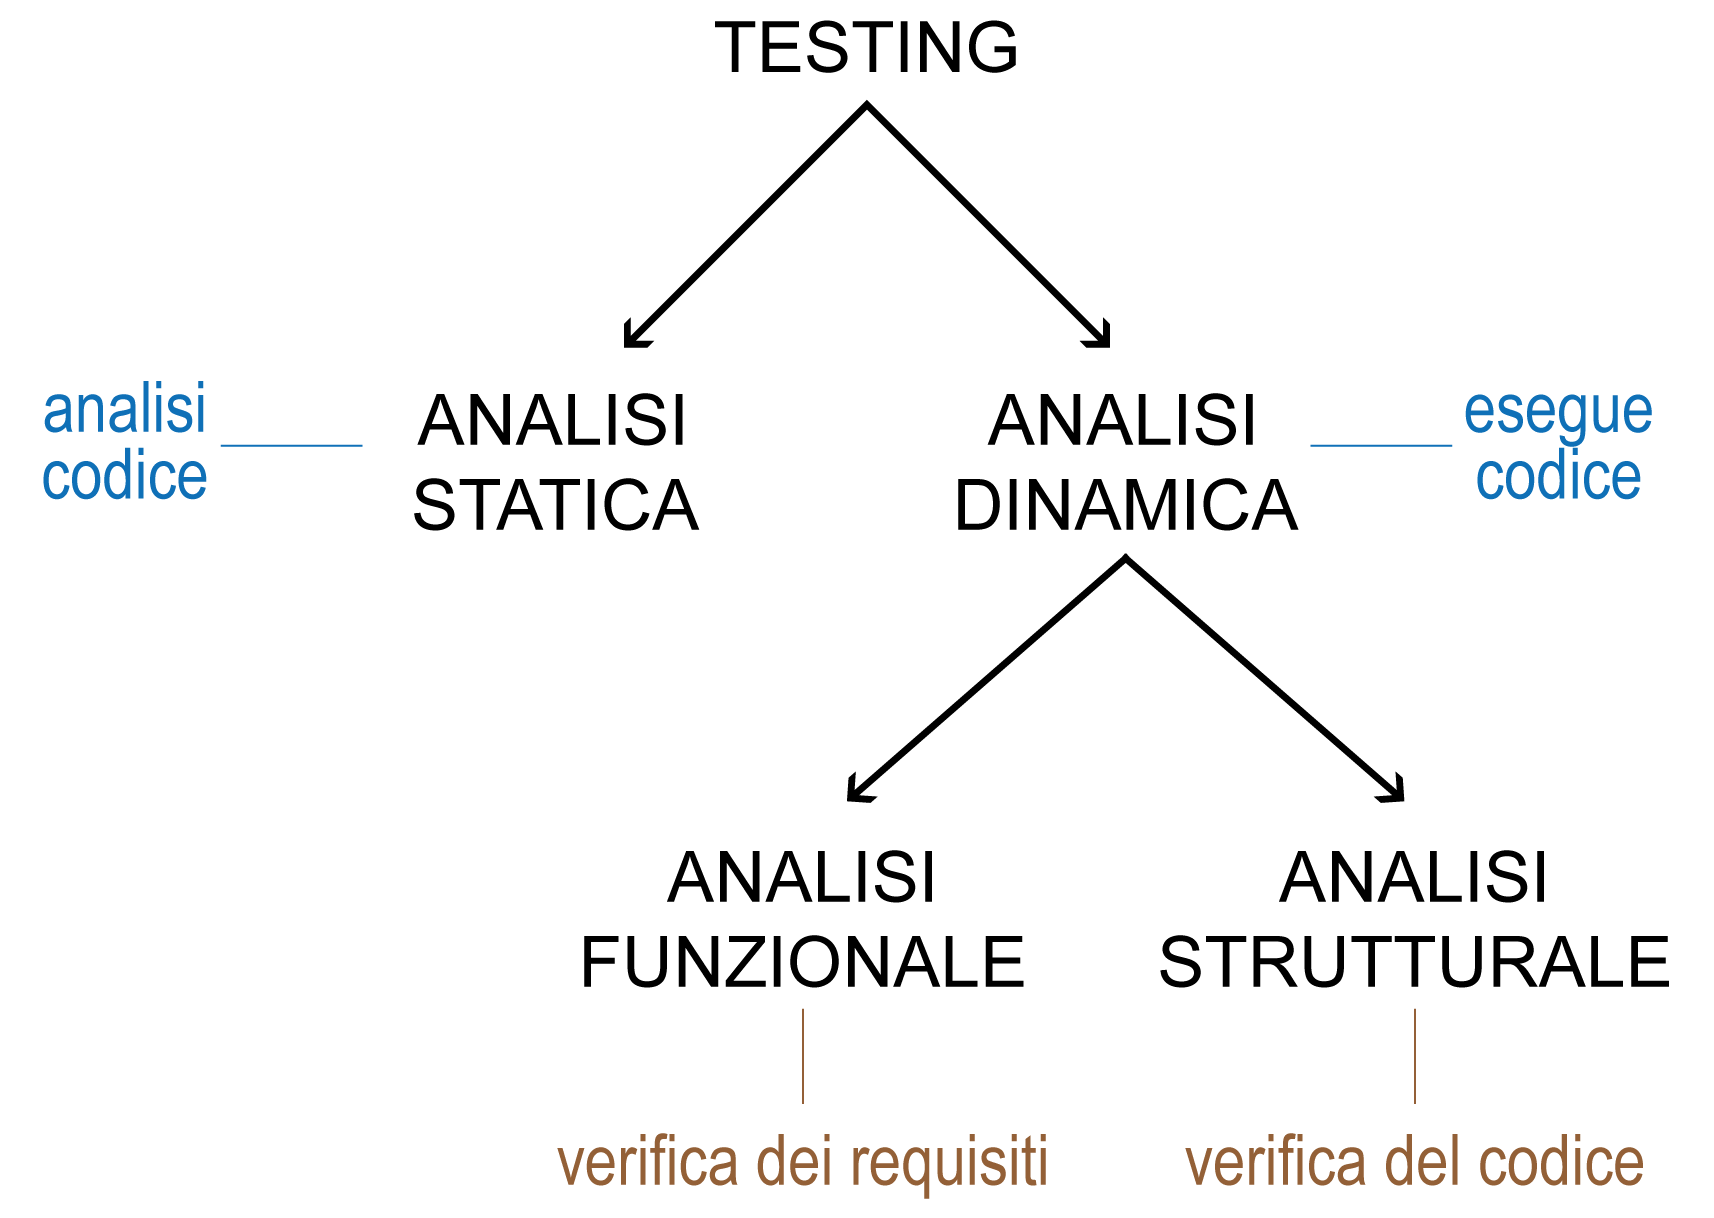
\includegraphics[scale=0.55]{img/testing.png}
\caption{I tipi di analisi del testing}
\label{fig:testing}
\end{figure}
\noindent
\newline
Un caso di test, per essere definito valido, deve avere un’alta probabilità di scoprire un errore, non essere ridondante, e garantire una verifica di giusta complessità.\\




\subsection{Testing con Jest}
\label{sec:jest}
Uno dei framework JavaScript più usati per il testing è Jest \cite{jest}, libreria che permette la creazione, l'esecuzione e la strutturazione dei test senza particolari configurazioni e include sia un test runner, che funzioni di asserzione. Fornisce anche una serie di funzionalità aggiuntive, come la ricerca automatica dei test da eseguire nel codice sorgente, l'esecuzione delle verifiche in parallelo o la possibilità di testare il codice asincrono in modo sincrono.\\
\newline
Nonostante non siano state elaborate verifiche tramite questa libreria durante il progetto, si riporta a titolo di esempio un possibile utilizzo per un test case banale \cite{jest_ex}. Il codice mostrato (listing \ref{code:jest}) presenta la funzione \verb|moltiplica| che riceve come parametri due numeri e ne effettua il prodotto, da questa si crea un file \verb|.js| contenente il test da verificare che, in questo caso, analizza la correttezza del risultato dell'operazione. Tramite Jest, dopo aver eseguito la prova, viene quindi restituito l'esito, positivo nel caso in cui il valore ritornato corrisponda alla corretta moltiplicazione e negativo viceversa con la prova che non viene considerata passata.

\begin{listing}[!hbt]
\begin{minted}{js}
//funzione moltiplica
function moltiplica(n1, n2) {
  return n1 * n2;
}
module.exports = moltiplica;

//creazione ed esecuzione test
const mul = require('./moltiplica');
test('mul 3 * 2 to equal 6', () => {
  expect(mul(3)(2)).toBe(6);
});

//risultato test
PASS  ./mul.test.js
OK mul 3 * 2 to equal 6 (5ms)
\end{minted}
\caption{Esempio di test con framework Jest}
\label{code:jest}
\end{listing}
\noindent



\subsection{Casi di test}
\label{sec:casi} 
Nonostante la fase di verifica tramite analisi dinamica non sia stata svolta tramite strumenti appositi, sono stati individuati vari test case verificati manualmente ispezionando le risposte di alcune funzioni critiche. Si riportano alcuni dei test effettuati relativi alla creazione dei profili utenti e di un'anagrafica (in questo caso quella dei \textit{Corsi} come esempio), illustrando precondizioni e risultato attesto, e riportandone il risultato effettivamente riscontrato.

\begin{table}[h!]
\centering
\begin{tabular}{|c|c|c|c|}
\hline
\multicolumn{1}{|c|}{\textbf{Caso di test}} & \multicolumn{1}{c|}{\textbf{Condizioni}} & \multicolumn{1}{|c|}{\textbf{Risultato Atteso}} & \multicolumn{1}{|c|}{\textbf{Risultato}}\\ \hline
Creazione di un account & \makecell{\textit{username} e\\ \textit{password}} &  \makecell{Il sistema crea l'account con le credenziali\\specificate e restituisce il messaggio \textit{OK}} &  \textit{OK} \\ \hline
\makecell{Creazione di un account\\senza specificare\\username e/o password} & --- & \makecell{Il sistema non crea l'account e restituisce\\il messaggio di errore \textit{err-user}} &  \textit{err-user} \\ \hline
\makecell{Creazione di un account\\senza rispettare\\i vincoli di password } & --- & \makecell{Il sistema non crea l'account e restituisce\\il messaggio di errore \textit{err-psw}} &  \textit{err-psw} \\ \hline

\end{tabular}
\caption{Casi di test su creazione account (tutti i test passati)}
\label{}
\end{table}

\begin{table}[h!]
\begin{center}
\begin{tabular}{|c|c|c|c|}
\hline
\multicolumn{1}{|c|}{\textbf{Caso di test}} & \multicolumn{1}{c|}{\textbf{Condizioni}} & \multicolumn{1}{|c|}{\textbf{Risultato Atteso}} & \multicolumn{1}{|c|}{\textbf{Risultato}}\\ \hline
Creazione di un corso & \makecell{campi\\obbligatori} &  \makecell{Il sistema crea il corso secondo i campi\\specificati e restituisce il messaggio \textit{OK}} &  \textit{OK} \\ \hline
\makecell{Creazione di un corso\\senza specificare tutti\\i campi obbligatori} & \makecell{---} & \makecell{Il sistema non crea il corso e restituisce\\il messaggio di errore \textit{err-corso}} &  \textit{err-corso} \\ \hline
\makecell{Eliminazione di un corso} & \makecell{vincoli di \\integrità\\rispettati}& \makecell{Il sistema elimina il corso e restituisce\\il messaggio \textit{OK}} &  \textit{OK} \\ \hline
\makecell{Eliminazione di un corso\\senza rispettare i\\vincoli di integrità} & \makecell{---} & \makecell{Il sistema non elimina il corso e restituisce\\il messaggio di errore \textit{err-contr}} &  \textit{err-contr}\\ \hline

\end{tabular}
\caption{Casi di test su creazione ed eliminazione corsi (tutti i test passati)}
\label{}
\end{center}
\end{table}

